\chapter{Chemical Bonds: Not Little Sticks}

\begin{kaichang}
\textbf{Translator safety note:} Treat the match and combustion examples as supervised demonstrations, not instructions to hold a burning match until heat reaches your hand. Do not prepare or ignite hydrogen/oxygen mixtures. Consult \href{https://institute.acs.org/acs-center/lab-safety/education-training/safer-experiments.html}{ACS demonstration safety guidance} and \href{https://www.energy.gov/cmei/fuels/safe-use-hydrogen}{DOE hydrogen precautions}.

Find a box of matches, take one out, and strike it.

Before blowing it out, watch carefully for three seconds: the chemicals on its head had been sitting quietly, as had the oxygen in the air, neither bothering the other. Yet one stroke against the box produces a little pop and a flame---light, heat, and enough burning heat to make you shake your hand.

Now make a guess: \textbf{who paid the bill} for that heat and light? Friction? You stopped rubbing long ago, but the flame keeps burning and releasing heat. The wood? Unlit wood feels cool. The air? Air surrounds you right now, yet you are not on fire.

Write down your guess. At the end of this chapter, we will return to this match and see that every bit of energy in its flame is a bill collectively settled by countless atoms as they ``join up.''
\end{kaichang}

\section{Visible Clues: Separation Takes Effort, Joining Releases Heat}

Let us not rush inside the atom. In the visible world, atoms' partnerships have two faces, both already familiar to you.

The first: \textbf{separating things that are joined takes effort}. You can snap a biscuit or a piece of chalk, but breaking iron wire with bare hands is almost impossible. Breaking cotton thread takes a hard pull with both hands. Even peeling apart two sticky notes requires some force. Separating partners is never free.

The second: \textbf{joining things often releases energy}. A burning match gives off heat and light. Ignite a mixture of hydrogen and oxygen and it releases a great burst of heat (which is why hydrogen is used as rocket fuel). Bring two magnets close and they snap together with a click---that sound is energy too. Joining is often when energy flows outward.

Together, these two faces suggest a clue: separating costs money; joining gives change back. Nature seems to keep a ledger recording the income and expenses of ``atoms joining and parting.'' Our job in this chapter is to open that ledger and learn its accounting rules.

\section{Zooming In: What Happens as Two Atoms Approach?}

From Chapter 9, we know that an atom consists of a tiny positive nucleus and a cloud of electrons arranged in energy levels. Now imagine two complete atoms slowly approaching from far apart. For simplicity, take hydrogen: one proton and one electron each.

Far apart, the atoms ignore each other. But once their electron ``clouds'' begin overlapping, \textbf{several forces change simultaneously}, and they do not all point the same way:

\begin{itemize}[itemsep=2pt]
\item Atom A's nucleus begins attracting atom B's electron, and B's nucleus attracts A's electron. Opposite charges attract, pulling the atoms together.
\item Meanwhile, the two positive nuclei repel each other, as do the two negative electron clouds. Like charges repel, pushing the atoms apart.
\end{itemize}

This is not a two-act play of ``attraction first, repulsion later,'' but \textbf{the simultaneous sum of every attraction and repulsion among all the particles}. The distance at which the atoms settle, and whether they join at all, depends not on any one force, but on whether all those forces together raise or lower the energy of the entire system.

This brings us to the chapter's central criterion. Underline it: \textbf{whether atoms bond depends not on ``who likes whom,'' but on the total energy of the whole system---all nuclei and all electrons. Bonding means that the system has found a lower-energy arrangement.}

Atoms have no wishes. They do not ``want'' stability or act ``to get eight electrons.'' They simply follow an almost boringly plain rule: if energy can move from high to low, it does---rather like water flowing downhill.

\section{One Curve Explains Bonding: An Energy Valley}

Plot the distance between two atoms against the system's total energy, and you get a curve shaped rather like a valley. This may be the most important diagram in this part:

\begin{center}
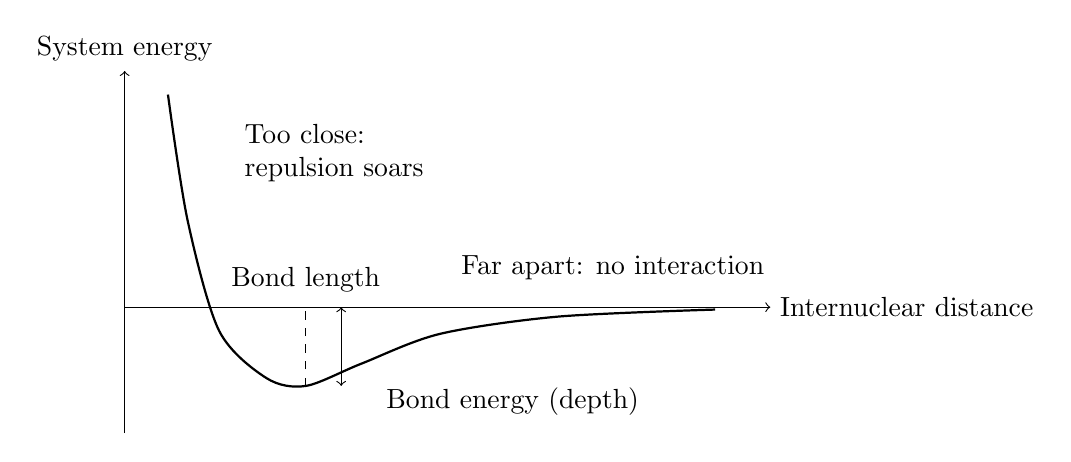
\begin{tikzpicture}[scale=1.0]
\draw[->] (0,0) -- (8.2,0) node[right]{Internuclear distance};
\draw[->] (0,-1.6) -- (0,3.0) node[above]{System energy};
\draw[thick] plot[smooth] coordinates {(0.55,2.7) (0.8,1.1) (1.2,-0.3) (1.8,-0.9) (2.3,-1.0) (3.0,-0.72) (4.0,-0.34) (5.5,-0.12) (7.5,-0.03)};
\draw[dashed] (2.3,-1.0) -- (2.3,0);
\draw[<->] (2.75,-1.0) -- (2.75,0);
\node[anchor=west] at (3.2,-1.2) {Bond energy (depth)};
\node at (2.3,0.35) {Bond length};
\node at (6.2,0.5) {Far apart: no interaction};
\node[anchor=west] at (1.4,2.2) {Too close:};
\node[anchor=west] at (1.4,1.75) {repulsion soars};
\end{tikzpicture}
\end{center}

(This is a schematic drawing. Neither axis gives actual scales for a particular molecule; it shows only the trend.)

Reading from right to left follows ``two atoms approaching'':

\begin{itemize}[itemsep=2pt]
\item \textbf{Far apart} (the right side): neither affects the other, so we set the system's energy to zero as our accounting baseline.
\item \textbf{Drawing closer}: nucleus--electron attraction begins to dominate, and total energy \textbf{falls}. Like water running downhill, the atoms approach spontaneously---provided their excess energy can be carried away.
\item \textbf{At the valley bottom}: at a particular distance, the balance of attraction and repulsion gives the lowest energy. This distance is the \textbf{bond length}; the energy needed to climb from the bottom back to zero (the valley's depth) is the \textbf{bond energy}.
\item \textbf{Squeezing closer}: repulsion grows sharply between nuclei and between electron clouds. Total energy turns upward, and the curve becomes almost vertical. Atoms are not soft fruit you can squeeze at will.
\end{itemize}

So what exactly is a chemical bond? It is \textbf{not} a little stick tying two atoms together. It is the fact that, at a particular separation, the system sits at an energy minimum. To keep the atoms away from the valley bottom, you must keep paying (doing work); once they fall in, they stay there on their own.

\begin{qiaoliang}
How large is a bond energy? Let us use real numbers. The \chem{H-H} bond in hydrogen has a bond energy of about \ud{436}{kJ\cdot mol^{-1}}: breaking the bonds in \ud{1}{mol} (that is, \ud{2}{g}) of hydrogen molecules costs 436 kilojoules. Per bond:

\[ \frac{436\times 10^{3}\ \mathrm{J}}{\ud{6.02\times 10^{23}}{mol^{-1}}} \approx 7.2\times 10^{-19}\ \mathrm{J} \]

A single bond's energy is less than a hundred-quadrillionth of a joule---pitifully small. Yet an ordinary match releases about \ud{1000}{J} of heat, equivalent to the energy released as roughly $10^{21}$ (one septillion) new bonds ``settle their accounts'' together. One atom's accounts are negligible, but when atoms act collectively by the mole, they produce a visible flame that can burn your fingers. This is the power of Avogadro's constant from Chapter 5: it exchanges the particle world's small change for our world's large bills.
\end{qiaoliang}

\section{Where Energy Comes From and Goes: Breaking Absorbs, Forming Releases}

Translate the curve into accounting language, and we get the sentence this chapter must get exactly right:

\textbf{Breaking chemical bonds requires energy absorption; forming chemical bonds releases energy.}

Do not reverse these directions. Breaking a bond pulls atoms out of the valley against attraction, requiring work, just as pulling apart two attached magnets takes effort. Forming a bond lets atoms drop into the valley, shedding excess energy as heat, light, and so on, just as magnets click when they snap together.

\begin{shiyan}
\textbf{Pulling Apart and Snapping Together: Exploring the ``Bond Ledger''}

Materials: two small magnets that attract each other (refrigerator magnets will do), a metal paper clip, and a dry spaghetti strand or piece of chalk.

Procedure: (1) Let the magnets stick together, then pull them apart, feeling the force your hands must exert. (2) Let them snap back together from your hands; listen closely for the click and touch the collision point. (3) Bend the paper clip back and forth. After several bends, immediately touch the bend---it is warm. Keep bending until it breaks, noticing the continuous work required beforehand. (4) Snap the spaghetti or chalk, paying attention to the crack: until the fracture appeared, your muscles were paying the bill.

What to observe: separating things that tend to join always takes effort (absorbs energy); joining and collisions release sound and heat (release energy). The warm bend in the paper clip shows that your work did not disappear: it became heat.

Safety note: use only small magnets to avoid pinched fingers. Do not point the paper clip toward anyone's eyes while bending it; broken ends are sharp. Wash your hands afterward. The forces here are macroscopic electromagnetic forces and bonding inside a metal. This is only an analogy for experiencing ``energy direction''; Chapters 18 and 21 explain the details.
\end{shiyan}

With this rule, chemical reactions become much clearer. Every reaction breaks old bonds (absorbing energy) and forms new ones (releasing energy). \textbf{Whether the reaction releases heat overall depends on the balance between the two}. Consider hydrogen burning in oxygen, using the bond-energy table coming shortly:

\[ \chem{2H_2} + \chem{O_2} \rightarrow \chem{2H_2O} \]

Breaking bonds costs: 2 lots of \chem{H-H} ($2\times 436$) plus 1 lot of \chem{O=O} (498), about \ud{1370}{kJ} altogether. Forming bonds returns: 4 lots of \chem{O-H} ($4\times 463$), about \ud{1852}{kJ}. Income exceeds expenditure, releasing about \ud{482}{kJ} net. This is only a rough estimate for gaseous water; actual combustion releases more heat. Rockets lift their enormous loads using this ``change returned by bonding.''

Conversely, splitting water back into hydrogen and oxygen reverses every payment. Water electrolysis therefore needs a continuous electricity supply: not a penny of energy can be skipped. No machine can ``turn water into fuel with a gentle touch.'' Anyone claiming otherwise is denying this ledger.

\section{Symbols: The Short Line Is Just an Accounting Mark}

Only now do we bring in the symbols. You have seen formulas like these:

\[ \chem{H-H} \qquad \chem{O=O} \qquad \chem{N\equiv N} \]

One short line between atoms denotes a single bond, two a double bond, and three a triple bond (Chapter 19 covers the details). Now you know these lines are \textbf{not} connectors drawn for atoms, but accounting symbols for humans. Each line says, ``There is an energy valley here, roughly this deep.''

Here are some common bond energies. The numbers are averages measured across different molecules; the same \chem{C-H} bond differs slightly between methane and alcohol:

\begin{table}[h]
\centering
\begin{tabular}{lclc}
\toprule
Bond & Energy ($\mathrm{kJ\cdot mol^{-1}}$) & Bond & Energy ($\mathrm{kJ\cdot mol^{-1}}$) \\
\midrule
\chem{H-H} & 436 & \chem{C-H} & 413 \\
\chem{C-C} & 347 & \chem{O-H} & 463 \\
\chem{O=O} & 498 & \chem{H-Cl} & 431 \\
\chem{N\equiv N} & 946 & \chem{Cl-Cl} & 243 \\
\bottomrule
\end{tabular}
\end{table}

A glance at the table explains several everyday facts. Nitrogen's \chem{N\equiv N} bond has an energy of \ud{946}{kJ\cdot mol^{-1}}, almost the deepest valley here. That is why the nitrogen making up four-fifths of the air passes through your lungs all day, taking part in almost no reactions, like a mild-mannered spectator. To ``split'' nitrogen into fertilizer crops can use, factories must attack this valley with high temperatures and pressures. This is the famous Haber process, which returns in Chapter 30 when we discuss reaction conditions. Oxygen is much more reactive: its \chem{O=O} bond energy is only about half nitrogen's. A shallower valley makes it easier to ``invite'' oxygen into reactions---one chemical reason breathing keeps you alive and fire can burn.

Greater bond energy means a deeper valley and a firmer partnership; a shallower valley means the partnership breaks up more easily. One table, half of chemistry.

\section{The Octet: A Useful Mnemonic, Not a Law}

In Chapter 10, we dismantled a widespread claim: ``Atoms react to get eight electrons.'' Energy language now lets us explain it properly.

The mnemonic ``a full outer shell of eight electrons is stable'' (the octet rule) is genuinely useful. Most common molecules made from main-group elements---water, carbon dioxide, methane, and the ions in table salt---obey it. There is a good reason: for second-period atoms such as carbon, nitrogen, oxygen, and fluorine, an arrangement with eight outer electrons often \textbf{happens} to correspond to the lowest-energy valley. The mnemonic is shorthand for an energy pattern.

But shorthand is not law. Once we bring in the real criterion, ``lowest total energy,'' exceptions immediately line up:

\begin{itemize}[itemsep=2pt]
\item \textbf{Stable with fewer than eight}: in boron trifluoride, \chem{BF_3}, boron has only 6 outer electrons, yet the molecule exists quite comfortably and is a common industrial reagent. Boron does not ``strive for eight,'' because under those circumstances the six-electron arrangement is already low enough in energy.
\item \textbf{Stable with more than eight}: sulfur in sulfur hexafluoride, \chem{SF_6}, has 12 electrons around it, while phosphorus in phosphorus pentachloride, \chem{PCl_5}, has 10. Atoms from the third period downward have larger ``floors'' that can accommodate more guests.
\item \textbf{Even an odd electron count is no obstacle}: nitric oxide, \chem{NO}, has an odd total number of electrons, so no allocation can give every atom eight paired electrons. Yet \chem{NO} exists stably and is an important signaling molecule in your blood vessels, helping regulate your blood pressure right now.
\item \textbf{Even the ``nobility'' gets involved}: noble gases have full outer shells and were once called ``inert gases''; textbooks declared that they never bonded. Yet chemists made \chem{XePtF_6} in 1962, followed by \chem{XeF_4} and other xenon compounds. If total energy can fall far enough, even a ``fully occupied'' floor can be remodeled.
\end{itemize}

The correct statement is therefore: \textbf{the octet is a useful empirical mnemonic; energy is the law behind it}. The mnemonic helps you quickly predict the structures of most common molecules. When exceptions appear, do not be surprised or feel sorry for atoms that ``failed to get eight.'' Their ledger never had an ``eight'' column, only a ``total energy'' column. In Chapter 19, drawing Lewis structures will bring you back to this mnemonic's limits repeatedly.

\section{How Scientists Know: From ``Little Sticks'' to Energy Curves}

\begin{zhengju}
The concept of a chemical bond arrived more than half a century before its explanation. Around 1858, Couper and Kekul\'e were already joining atoms with short lines in structural formulas. Those lines were remarkably useful, explaining how carbon could build such varied frameworks. Yet nobody could say what a line really represented. A hook sticking out of an atom? Nobody had seen one.

In 1916, the American chemist Lewis proposed a bold guess: bonding involved two atoms \textbf{sharing a pair of electrons}. This explained the composition of many molecules and gave rise to the octet rule. But an immediate objection arose: two negatively charged electrons repel each other, so why should bringing them together glue atoms together? It sounded counterintuitive, and Lewis could not supply a calculation.

The real answer awaited quantum mechanics. In 1927, the year after the Schr\"odinger equation appeared, two young physicists working in Germany, Heitler and London, undertook an extraordinarily difficult calculation. Treating both nuclei and electrons of two hydrogen atoms as a quantum system, they calculated how the whole system's energy varied with internuclear distance. The curve had a clear minimum: the valley at the start of this chapter emerged from theory for the first time. Their predicted bond length and energy broadly agreed with experiment. More importantly, their calculation showed that \textbf{classical electrostatic attraction alone could never produce such a valley}. Bonding is fundamentally quantum-mechanical. Roughly speaking, sharing gives the electrons more room to move, lowering their kinetic energy (see the challenge box). Pauling and others later extended these ideas to many molecules, turning ``chemical bonding = lower system energy'' from a guess into a calculable, testable theory.

Experimenters were busy too. The Braggs directed X-rays through crystals and inferred atomic separations from diffraction patterns, ``measuring'' bond lengths for the first time. The infrared frequencies absorbed by molecular vibrations revealed how stiff the bond ``springs'' were, indirectly weighing their bond energies. Agreement between calculated valley depths and experimental measurements put the picture on firm ground. Notice the sequence: accounting symbols (1858), a conjecture (1916), then an explanation (1927) and independent measurements (diffraction and spectroscopy). Science was not a relay of geniuses' sudden insights, but nearly a century of symbols, guesses, calculations, and measurements checking one another.
\end{zhengju}

\section{When This Model Breaks Down}

Potential-energy curves and bond-energy tables are enormously useful tools, but you deserve to know their boundaries before they mislead you.

First, the curve treats nuclei as little balls at definite positions---a classical picture. In reality, electrons spread around nuclei as probability clouds (Chapter 9). Bond length is only the most probable separation; atoms constantly vibrate near the valley bottom and never sit still.

Second, bond-energy tables give \textbf{averages}. An \chem{O-H} bond in water is not quite the same ``quality'' as one in alcohol. Reaction heats calculated from a table are reasonable estimates, not exact accounts.

Third, the ``one line, one bond'' system cannot record whole categories of transactions. The bonds between benzene's 6 carbons are neither single nor double, but an evenly distributed ``one and a half.'' In copper metal, there is no particular pair of atoms joined together; the whole metal shares its electrons (Chapter 21). The weak but important attractions between molecules---why water forms a flowing liquid, or why geckos climb walls---are not in this bond-energy table at all (Chapter 22). In such cases, the stick model is not ``calculating incorrectly''; the transactions simply fall outside its scope.

\begin{wuqu}
``Chemical reactions release energy because chemical bonds break.'' This is one of chemistry's most widespread errors, with the direction completely reversed.

Counterexamples are easy to find. If breaking bonds released energy, pulling iron wire apart should \textbf{release} heat. Yet when you bend a paper clip until it breaks, the bend warms, the fracture does not burst into flame, and you must keep applying force. If breaking bonds released energy, water molecules should fall apart into hydrogen and oxygen on their own and generate electricity, instead of requiring electricity to split them.

Energy is released at only one point: \textbf{when atoms fall into an energy valley and new bonds form}. A burning fuel releases heat not from ``old bonds breaking,'' but from ``new bonds returning change.'' The products' bonds (in \chem{CO_2} and \chem{H_2O}, for example) are deeper and more stable than the reactants' bonds. The net profit after balancing the accounts is the heat you feel. Whenever you encounter claims that ``breaking high-energy bonds releases energy''---including some popular explanations of ATP, which Chapter 46 will scrutinize---automatically redo the accounts in your head.
\end{wuqu}

\section{Back to the Match}

Now let us keep our promise and work through that match's accounts, entry by entry.

When you strike the side of the box, friction does work, handing a little energy to the match-head chemicals. Its purpose is specific: \textbf{paying the first bond-breaking bill}. Old bonds in the chemicals and the air are pried apart, lifting atoms out of their valleys.

Then the main act begins: these ``freed'' atoms form new partnerships and plunge into deeper valleys. Carbon and oxygen form \chem{CO_2}; hydrogen and oxygen form \chem{H_2O}. New bonds form, and \textbf{bond formation releases energy}. The new valleys are much deeper than the old, and the returned change pours out as heat and light, burning your fingers and illuminating the flame. It also heats neighboring chemicals until they can ``afford the bond-breaking bill,'' sustaining the flame until the chemicals are used up.

Fire is therefore \textbf{a chain of transactions started with an upfront payment and sustained by change returned from bonding}. The frictional work of striking a match is only the ``ignition fee''; the real fuel is the energy difference between chemical bonds. This also answers our opening puzzles. Cool wood releases no heat because its atoms sit quietly in their valleys. Air does not burn you because even the relatively shallow \chem{O=O} valley requires someone to pay the initial ``bond-breaking deposit.''

And why is iron wire so hard to break? Metal atoms do not pair off; they all share a vast pool of ``public electrons,'' making the whole metal one enormous energy valley. That is another accounting system, covered in Chapter 21.

\section{Digging Deeper: Where Does This Ledger Lead?}

``Breaking absorbs, forming releases'' explains far more than matches. It is the chief accountant of the energy world. Coal, oil, and natural gas are fuels because rearranging their chemical bonds releases energy overall. Batteries arrange for that bill to be paid gradually as electric current. Explosives and ordinary fuels have exactly the same accounts; the difference is the \textbf{speed} of settlement, a question of kinetics answered in Chapter 28. Your body works the same way: food and inhaled oxygen ultimately balance their accounts in this ledger, paying for body temperature, heartbeats, and thought. Life's accounting is much more sophisticated, though, and will unfold gradually in Volume Three.

So far, however, we have established only the general reason atoms join, without examining the very different ways they do it. Next chapter, we watch the most decisive kind: when sodium meets chlorine, electrons are not shared but \textbf{transferred outright}. A sodium atom loses an electron completely; a chlorine atom takes it completely; the resulting charged ions gather through electrostatic attraction. This ``transfer first, embrace afterward'' bonding explains why salt is hard yet vulnerable to water, why its melting point is high enough for crucible material, and why it can light a lamp. Turn to Chapter 18 to see what happens after electron ownership changes.

\begin{tiaozhan}
(You can skip this without losing the main thread.) Why can sharing electrons lower energy? A rough picture lies within Heitler and London's calculation. In quantum mechanics, an electron's energy has two parts: potential energy lowered by attraction to nuclei, and kinetic energy related to its ``room to move.'' The more tightly confined an electron is, the higher its kinetic energy---like a ping-pong ball bouncing more vigorously in a smaller room. As two hydrogen atoms approach, each electron can appear near either nucleus: more room lowers kinetic energy, while proximity to both positive nuclei lowers potential energy. Together, these two credits outweigh nuclear repulsion and produce the valley. More precisely, kinetic and potential energy trade off during bonding and ultimately obey a strict relationship called the ``virial theorem.'' A small region near the valley bottom can also be approximated as a spring (a parabola), while a ``Morse potential'' such as $E(r)=D\left(1-e^{-a(r-r_0)}\right)^2$ fits the whole curve. Molecular infrared spectra measure this ``spring's'' vibration frequency to infer the bond's stiffness.
\end{tiaozhan}

\section*{Try It}

\begin{sikaoti}
\item Without looking at the book, draw the system's energy as a function of distance for two approaching atoms. Label the zero at infinite separation, bond length, bond energy, and why the curve rises when the atoms are ``too close.'' Explain in one sentence why atoms ``spontaneously'' settle at the bottom.
\item Use this chapter's table to determine whether $\chem{H_2} + \chem{Cl_2} \rightarrow \chem{2HCl}$ releases or absorbs heat. What is the total cost of breaking bonds, the return from forming them, and the final balance? (Hint: the \chem{H-Cl} bond energy is \ud{431}{kJ\cdot mol^{-1}}.)
\item Someone says, ``Explosives are powerful because their molecules store many high-energy bonds, which break during an explosion and release energy.'' Identify two directional errors and use ``valley'' language to explain why explosives release energy.
\item Nitrogen, \chem{N_2}, makes up about four-fifths of air but rarely reacts; oxygen, \chem{O_2}, makes up only a fifth but supports combustion. Use the bond-energy table to explain their different ``personalities,'' and what this difference means for your ability to breathe safely.
\item Sulfur has 12 surrounding electrons in \chem{SF_6}, while boron has only 6 in \chem{BF_3}. Using ``the octet is a mnemonic; energy is the law,'' write a paragraph explaining their stable existence to a friend convinced that ``atoms must have eight electrons.''
\end{sikaoti}
